\chapter{Implementacja aplikacji}
Rozdział poświęcony jest opisowi aplikacji, które zostały stworzone na potrzeby pracy.
Na podstawie ich implementacji wysuwane są wnioski w kolejnym rozdziale.

\section{Opis domeny}
Domena problemowa, którą wybrał autor pracy do zaimplementowania, jest bardzo prosta ideowo i biznesowo. Jest to aplikacja internetowa, w której można wystawiać i sprzedawać karty podarunkowe.

Istnieją trzy rodzaje użytkowników:
\begin{itemize}
    \item Kupujący,
    \item Sprzedający,
    \item Administrator.
\end{itemize}

Główną encją, na której przeprowadzane są operacje w systemie to karta podarunkowa. 
Każda karta podarunkowa musi mieć markę (ang. brand), cenę sprzedaży, wartość rynkową, datę ważności i kod do wykorzystania w sklepie. Karta może być fizyczna lub elektroniczna. Na podstawie ceny wyznacza się przedział cenowy (ang. price range) w której się znajduje.

Operacje, które mogą być wykonywane w systemie to:
\begin{itemize}
    \item Zaawansowane wyszukiwanie z filtrami i sortowaniem branż, wraz z ich aktualną maksymalną zniżką. Operacja przeznaczona dla kupującego.
    \item Zaawansowane wyszukiwanie z filtrami i sortowaniem listy dostępnych kart wg marek, do których należą. Operacja przeznaczona również dla kupującego.
    \item Lista i filtrowanie wszystkich kart i transakcji dla administratora.
    \item Weryfikacja karty przez administratora. Dopiero po weryfikacji karta pojawia się w systemie sprzedaży.
    \item Operacje zamówienia (określana jako ,,checkout'') i zapłaty (określana jako ,,pay'') karty przez kupującego. Sprzedający może taką operację widzieć w systemie odpytując listę transakcji, w których bierze udział.
    \item Operacja wysyłki karty przez sprzedającego do kupującego.
    \item Lista wszystkich transakcji dla zarówno kupującego jak i sprzedającego, w których biorą udział.
    \item Możliwość edycji i usuwania marki i karty przez administratora.
    \item Możliwość edycji i usuwania karty, którą sprzedający umieścił w systemie.
\end{itemize}

\section{Implementacja wersji opartej na monolicie z anemicznym antywzorcem}
Pierwszym i najbardziej naturalnym podejściem do zaimplementowania domeny problemowej opisanej powyżej jest stworzenie aplikacji monolitycznej\index{aplikacja monolityczna} opartej na relacyjnej bazy danych. Wszystkie operacje w systemie mają odzwierciedlenie na encji bazy danych jaką jest karta podarunkowa. 

Takie podejście jest dla większości programistów pierwszym wyborem, jeżeli myśli się o szybkiej implementacji systemu i walidacji pomysłu jako MVP (ang. minimal value product). Większość frameworków w różnych językach programowania opiera się własnie na tym modelu. 

Dodatkowo, aplikacja została napisana w sposób anemiczny\index{Anemic Model}, czyli jest to tak naprawdę zastąpienie manualnego pisania zapytań bazodanowych poprzez dodatkową warstwę aplikacji, która jest pewnego rodzaju interfejsem dla użytkownika do wykonywania operacji.

Implementacja opiera się na Javie w wersji 10 i Spring\index{Spring} Framework. Użyte zostały moduły Spring Boot i Spring Data.

\subsection{Diagram bazy danych}
Diagram przedstawia relacje między encjami, które opisują zakładaną domenę problemową. Na tej strukturze bazodanowej opera się omawiana implementacja aplikacji.
Głównymi encjami jest marka (ang. brand), karta (ang. card) i transakcja (ang. transaction) i użytkownik (ang. user).

Operacje zakupu i wysyłki kart opierają się na encji transakcji, zawierająca aktualny stan (np. zainicjowana).

\begin{figure}[h!]
  \centering
    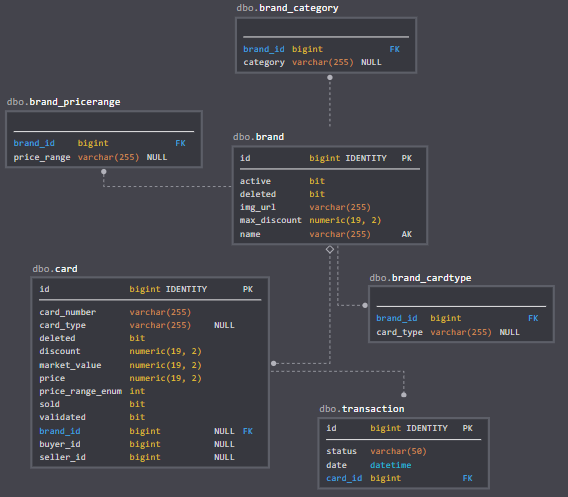
\includegraphics[width=1.0\textwidth]{images/modelERP.PNG}
  \caption{Diagram bazy danych. Źródło: opracowanie własne }
\end{figure}
\FloatBarrier


\subsection{Organizacja kodu}
Kod został logicznie podzielony na pakiety (ang. packages), gdzie więszkość pakietów znajdujących się w pl.cba.gibcode.alabackend odpowiada za typ encji i wszystkie operacje z nią związane.
Możemy wyróżnić nastepujące pakiety w lokalizacji pl.cba.gibcode.alabackend:
\begin{itemize}
    \item brand - wszystkie operacje na marce karty,
    \item card - wszystkie operacje dotyczące kart,
    \item transaction - wszystkie operacje na transakcjach,
    \item user - wszystkie operacje na użytkownikach,
    \item config - wszystkie klasy konfiguracyjne (np. konfiguracja Swaggera)
    \item shared - wspólny kod zawierający wszystkie modele w aplikacji, które są używane w wielu miejscach na raz,
    \item schedule - scheduler, który w równomiernym przedziale czasowym wymusza czyszczenie kart, które zostały kupione, ale nie zostały zapłacone w danym okresie czasu,
    \item startup - skrypt tworzący przykładową populację danych w bazie danych podczas włączania aplikacji.
\end{itemize}

Każda z ww. pakietów związanych z daną encją (tj. brand, card, transaction i user) posiada zbliżoną strukturę, składającą się z logicznego podziału:
\begin{itemize}
    \item filter - wszystkie klasy tworzące filtry do zapytań wg kryteriów tworzonych po stronie REST Api,
    \item mapper - pakiet ze wszystkimi mapowaniami między obiektami encji, a obiektami, które są odpowiedzią lub zapytaniem REST Api,
    \item model - definicje klas wszystkich modeli dotyczących danej encji,
    \item repository - repozytoria encji używające moduł Spring\index{Spring} Data,
    \item service - tzw. serwisy, które dokonują zmian na encjach, zmieniają ich stan, który zapisują poprzez repozytoria,
    \item web - miejsce na kontrolery REST Api używające Spring\index{Spring} MVC Rest Controllers.
\end{itemize}
\begin{figure}[!htb]
  \centering
    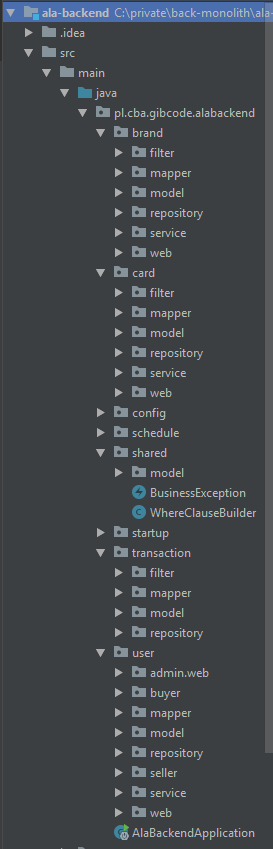
\includegraphics[width=0.4\textwidth]{images/monolit-structure.PNG}
  \caption{Struktura aplikacji monolitycznej. Źródło: opracowanie własne }
\end{figure}
\FloatBarrier

\subsection{Repozytoria encji}
Repozytoria encji oparte są na Spring\index{Spring} Data i są fasadami umożliwiającymi odczyt i zapis danych w bazie danych. Dla każdej encji istnieje osobne repozytorium. Do zdefiniowanych repozytoriów należą:
\begin{itemize}
    \item BrandRepository
    \item CardRepository
    \item TransactionRepository
    \item UserRepository
    \item UserDetailsRepository
\end{itemize}
\subsection{Połączenie z bazą danych}
Aplikacja opiera się na Hibernate jako ORM (ang. object-role modeling), gdzie sama implementacja bazy danych jest dowolona (może być to serwer mySql, PostgreSql, czy jakikolwiek inny relacyjny silnik bazodanowy). W aktualnej wersji projektu domyślnie aplikacja opiera się na bazie danych w pamięci H2. Za każdym resetowaniem aplikacji, baza danych zostaje zupełnie czyszczona i odtwarzana ponownie. W aplikacji autor pracy zamieścił automatyczne skrypty, które wstępnie ładują przykładowe dane do bazy danych, na których można wykonywać następnie operacje.

\begin{figure}[h!]
  \centering
    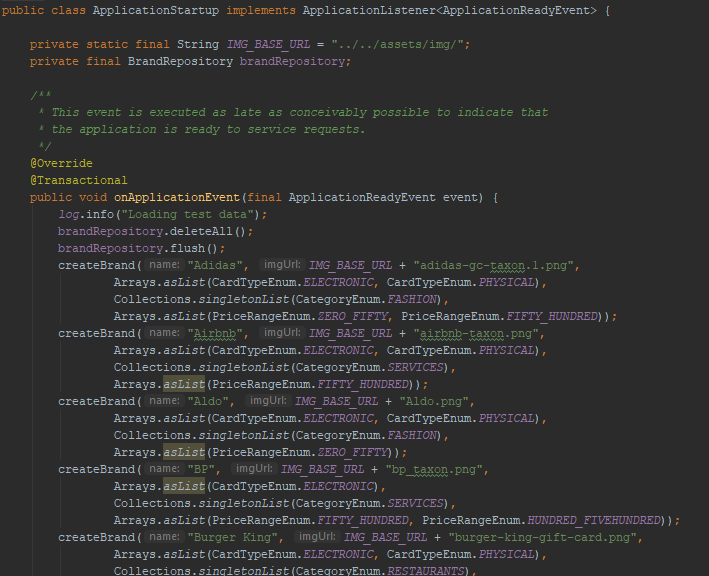
\includegraphics[width=1.0\textwidth]{images/script.PNG}
  \caption{Fragment klasy ładującej dane przy włączaniu aplikacji. Źródło: opracowanie własne }
\end{figure}
\FloatBarrier

\subsection{REST'owe enpointy}
Każda z funkcjonalności opisana w domenie aplikacji jest dostępna przez REST Api udostępniane z aplikacji. Funkcjonalności zostały pogrupowane wg encji. Dla każdej encji stworzono kontroler z nią pozwiązany.

\begin{figure}[h!]
  \centering
    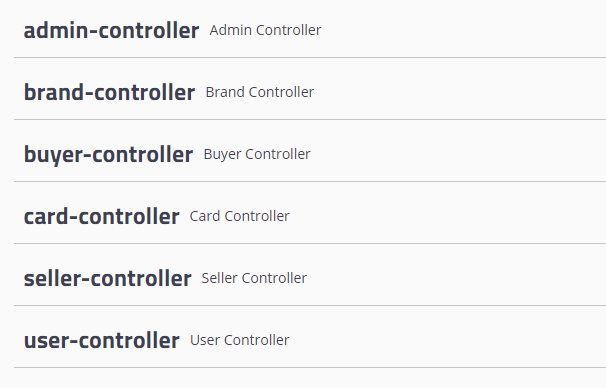
\includegraphics[width=1.0\textwidth]{images/controllerlist.PNG}
  \caption{Lista kontrolerów w aplikacji. Źródło: opracowanie własne }
\end{figure}
\FloatBarrier


\subsubsection{Kontroler administratora}
Kontroler dla administratora składa się z następującej listy endpointów:
\begin{itemize}
    \item admin/brands z metodą HTTP GET - lista wszystkich marek dla administratora,
    \item admin/brands z metodą HTTP PUT - edycja marki,
    \item admin/brands z metodą HTTP DELETE - usunięcie marki,
    \item admin/cards z metodą HTTP GET - lista wszystkich kart,
    \item admin/cards z metodą HTTP DELETE - usunięcie danej karty,
    \item admin/cards/validate - walidowanie danej karty,
    \item admin/users - lista wszystkich użytkowników.
\end{itemize}
\begin{figure}[h!]
  \centering
    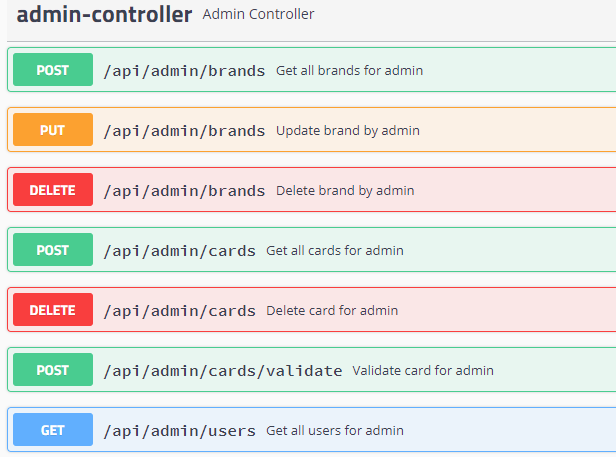
\includegraphics[width=1.0\textwidth]{images/admin-controller.PNG}
  \caption{Endpointy kontrolera administratora. Źródło: opracowanie własne }
\end{figure}
\FloatBarrier

\subsubsection{Kontroler marki}
Kontroler marek (ang. brands) składa się z następującej listy endpointów:
\begin{itemize}
    \item brands/create - tworzenie nowej marki,
    \item brands/list - lista wszystkich dostępnych marek (takie, które zawierają choć jedną kartę na sprzedaż).
\end{itemize}
\begin{figure}[h!]
  \centering
    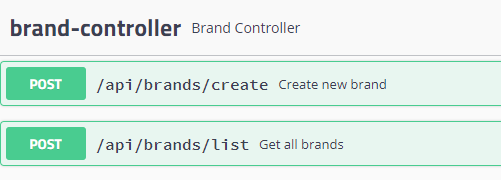
\includegraphics[width=1.0\textwidth]{images/brand-controller.PNG}
  \caption{Endpointy kontrolera marek. Źródło: opracowanie własne }
\end{figure}
\FloatBarrier

\subsubsection{Kontroler kupującego}
Kontroler kupującego (ang. buyer) składa się z następującej listy endpointów:
\begin{itemize}
    \item buyer/checkout - podsumowanie zakupu karty (jeszcze przed zapłatą)
    \item buyer/pay - kupujący płaci za utworzoną transakcję przy buyer/checkout
    \item buyer/transactions - lista wszystkich transakcji kupującego
\end{itemize}
\begin{figure}[h!]
  \centering
    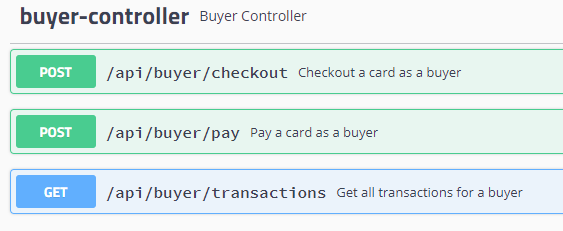
\includegraphics[width=1.0\textwidth]{images/buyer-controller.PNG}
  \caption{Endpointy kontrolera kupującego. Źródło: opracowanie własne }
\end{figure}
\FloatBarrier

\subsubsection{Kontroler kart}
Kontroler kart składa się z jednego endpointu:
\begin{itemize}
    \item cards/list - lista kart dostępnych do sprzedaży
\end{itemize}
\begin{figure}[h!]
  \centering
    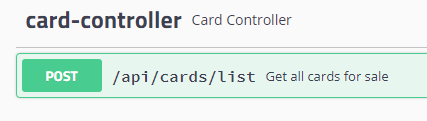
\includegraphics[width=1.0\textwidth]{images/card-controller.PNG}
  \caption{Endpointy kontrolera kart. Źródło: opracowanie własne }
\end{figure}
\FloatBarrier
\subsection{Uruchomienie aplikacji}
Aby uruchomić aplikację trzeba zainstalować Apache Maven w wersji 3.
Po tym, w głównym folderze z kodem źródłowym należy podać komendę w terminalu ,,mvn spring-boot:run''. Ta komenda spowoduje, że aplikacja zostanie zbudowana i wystartuje na wbudowanym serwerze aplikacyjnym Tomcat na porcie 8080.

Aplikacja po uruchomieniu powinna być dostępna na \url{http://localhost:8080/alakarta/swagger-ui.html}
Jest to strona z interfejsem udostępnionym przez Swaggera, gdzie można wykonywać interaktywne zapytanie do udostępnionego REST Api.


\section{Implementacja wersji opartej na Event Sourcing'u}
Coraz bardziej modnym podejściem staje się oparcie aplikacji o Event Sourcing.\index{Event Sourcing} Z autopsji autora tekstu i jego kariery programistycznej wynika, że coraz częściej wybierane jest właśnie to podejście, zwłaszcza w aplikacjach bankowych, gdzie każda transakcja musi zostać zapisana dla zachowania całej historii aplikacji. 

Nie dziwi też fakt, iż takie rozwiązania stają się coraz bardziej popularne, zwłaszcza, że jesteśmy w czasach rozkwitu technologii opartych o Blockchain. Idea zapisywania historii wszystkich wydarzeń jest zbliżona do Blockchain.

Event Sourcing\index{Event Sourcing} z natury opiera się na mikroserwisach i tak też jest w wypadku implementacji obranej domeny problemowej.

\subsection{Event Sourcing w Apache Kafce}
Event Sourcing\index{Event Sourcing} został zaimplementowany za pomocą Apache Kafka.
Amerykańska firma Confluent, najbliższy partner i firma konsultingowa technologii Apache Kafka, poleca użycie tej technologi do Event Sourcing'u\index{Event Sourcing}, pisząc:

,,Event Sourcing\index{Event Sourcing} i Apache Kafka są powiązane. Event Sourcing obejmuje utrzymywanie niezmiennych sekwencji zdarzeń, które mogą subskrybować wiele aplikacji. Kafka to wysokowydajny, o niskiej latencji, skalowalny i trwały dziennik, który jest używany przez tysiące firm na całym świecie i jest testowany na skalę bitewną. W związku z tym Kafka jest naturalnym kręgosłupem do przechowywania wydarzeń przy przechodzeniu do architektury aplikacji opartej na pozyskiwaniu zdarzeń.'' \cite{Confluent}

\subsubsection{Persystencja wydarzeń}
Wszystkie wydarzenia w aplikacji zostają zapisane przez Kafkę do plików systemowych, dzięki czemu nie ma potrzeby integracji z jakąkolwiek inną bazą danych jak np. w przypadku aplikacji monolitycznej.\index{aplikacja monolityczna}

\subsubsection{Wydarzenie jako Order}
Każde wydarzenie w aplikacji zostało przyporządkowane danej akcji i typowi wydarzenia, które może się powieść lub nie zostać zrealizowane. Dlatego każde wydarzenie jest jednoczenie traktowane jako swoiste zamówienie (ang. order), które ma swój identyfikator UUID. 

Zobrazuje to przykład kupna karty. Z jednej strony stan danych zostanie zmieniony podczas realizacji zamówienia, a z drugiej możemy sprawdzić jako kupujący, czy wszystko powiodło się. Sprzedający mógł wycofać w międzyczasie kartę z systemu i zamówienie mogło zostać przerwane, o czym kupujący zostanie powiadomiony jak tylko wyśle zapytanie o dany ,,order''.

Każde wydarzenie ma strukturę obiektową podzieloną na nagłówek i główne ciało. W nagłówku znajduje się informacja nt. akcji jaką ma wydarzenie wykonać i jej typ. W ciele głównym wydarzenia znajdują się szczegóły zamówienia, gdzie np. przy tworzeniu nowej karty znajdują się tu jej wszystkie potrzebne szczegóły.

Zdefiniowano dwa typy wydarzeń, tj. zamówienia dot. kart i marek.

Wszystkie możliwe akcje zamówień dot. marek to:
\begin{itemize}
    \item Tworzenie marki
    \item Aktualizacja marki
    \item Usunięcie marki
\end{itemize}

Lista akcji zamówień dot. kart:
\begin{itemize}
    \item Tworzenie karty
    \item Aktualizacja karty
    \item Usunięcie karty
    \item Walidacja karty
    \item Podsumowanie zamówienia karty przed płatnością
    \item Opłacenie zamówionej karty
    \item Wysłanie karty
\end{itemize}


\subsubsection{Maszyna stanów}
Dzięki traktowaniu każdego wydarzenia jako zamówienia posiadającego akcję i typ, możemy sprecyzować stan w jakim znajduje się aktualnie dana encja przed i po realizacji zamówienia. Jest to typowy automat skończony (ang. finite state machine), czyli abstrakcyjny, matematyczny, iteracyjny model zachowania systemu dynamicznego oparty na tablicy dyskretnych przejść między jego kolejnymi stanami. \cite{AutomatSkonczony}

Posiadanie informacji o stanie encji pozwala na wprowadzenie logiki do walidacji akcji, które są wykonywane na encji.
Dobrze zobrazuje to sytuacja w której karta nie może zostać kupiona, jeżeli nie jest zweryfikowana uprzednio przez administratora. Innym przykładem byłaby sytuacja, gdzie karta została już kupiona. W tej sytuacji możliwy następujący stan to jedynie wysyłka karty. Karta na tym etapie nie może już zostać usunięta ani kupiona przez innego użytkownika.

\subsection{Podział na mikroserwisy wg wzorca CQRS}
Aplikacja została podzielona na trzy mikroserwisy zgodnie z założeniami wzorca CQRS.\index{CQRS} Jeden mikroserwis odpowiedzialny jest za dokonywanie zmian w systemie, a inny za czytanie stanu danych. Oba posiadają dostępne REST-owe endpointy HTTP. Trzecim mikroserwisem jest silnik zamówień, nie posiadający dostępnyego REST Api, a który posiada logikę biznesową i jest implementacją wspomnianej już maszyny stanów.

\begin{itemize}
    \item ,,apiCommand'' posiadający wystawiony REST Api, przeznaczony do wysyłania komend (ang. command), dokonujących zmian w danych aplikacji,
    \item ,,apiQuery''posiadający wystawiony REST Api, przeznaczony do wysyłania zapytań (ang. query), bez możliwości edycji danych,
    \item ,,orderComponent'' odpowiedzialny za przyjmowanie zamówień (ang. order) od apiCommand i stałe przetwarzanie strumieni danych, które następnie mogą być odpytywane przez apiQuery.
\end{itemize}


\subsection{Połączenie z Apache Kafka}
Wszystkie wymienione wyżej mikroserwisy komunikują się między sobą za pomocą połączenia z serwerem Apache Kafka, wspólnym dla każdej aplikacji. Kafka jest wykorzystana jednocześnie jako baza danych i jako audyt wszystkich wydarzeń, zaszłych w systemie. Mikroserwis orderComponent jako jedyny komunikuje się tylko i wyłącznie poprzez Kafkę z pozostałymi mikroserwisami w środowisku. Jednakże jest to komunikacja jednostronna, gdzie zarówno apiCommand jak i apiQuery wysyłają wydarzenia dla orderComponent, u którego nie ma potrzeby wysyłki odpowiedzi lub innych zapytań poprzez wydarzenia w drugą stronę.

\section{Struktura aplikacji apiCommand}
Aplikacja apiCommand odpowiada za interakcję z interfejsem użytkownika poprzez przyjmowanie zapytań HTTP. Wystawiony jest własny REST Api. Po przyjęciu zapytania HTTP, po uprzednim zwalidowaniu, zostaje stworzone wydarzenie w aplikacji i wysyłane do serwera Apache Kafka. Każde takie wydarzenie jest odbierane przez orderComponent. Zgodnie z ideą CQRS\index{CQRS}, ten mikroserwis odpowiada za wysyłanie komend, dokonujących zmian w danych całego systemu.

\subsection{Organizacja kodu}
Każdy z trzech mikroserwisów posiada podobną strukturę, gdzie:

\begin{itemize}
    \item ,,config'' zawiera wszystkie pliki konfiguracyjne,
    \item ,,model'' zawiera wszystkie modele obiektów używane tylko i wyłącznie przez ten mikroserwis. Pozostałe modele wspólne są w osobnym module modelLibrary,
    \item ,,service'' zawiera tzw. serwisy, czyli klasy posiadające logikę biznesową np. usuwanie karty z systemu, 
    \item "web" to pakiet z kontrolerami Springowymi\index{Spring} udostępniającymi zasoby przez REST Api.
\end{itemize}


\begin{figure}[h!]
  \centering
    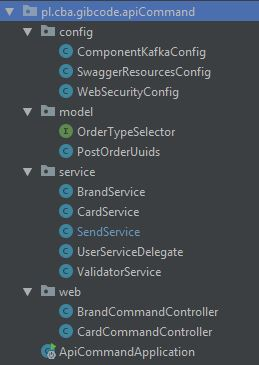
\includegraphics[width=0.5\textwidth]{images/apiCommand_packages.JPG}
  \caption{Organizacja kodu w apiCommand. Źródło: opracowanie własne }
\end{figure}
\FloatBarrier

\subsection{Walidacja zapytań}
Każde zapytanie, które zostaje odebrane przez mikroserwis zostaje zwalidowane, zanim zostanie stworzone wydarzenie przekazywane do brokera Kafka. Walidacja zostaje zrealizowana poprzez wyciągnięcie informacji z Apache Kafka o danej encji karty lub marki. Zapytanie skierowane do Apache Kafka jest oparte na wydobyciu danego obiektu na podstawie klucza encji, jakim jest jej ciąg znaków UUID. Realizacja takiego zapytania jest umożliwiona dzięki wykorzystaniu API udostępnionego przez Kafka Streams. Został użyty ReadOnlyKeyValueStore z pakietu org.apache.kafka.streams.state, który umożliwia zapytanie o wydarzenia z serwera Kafki na podstawie ich kluczy, zakresu kluczy jeżeli są one tworzone w sposób sekwencyjny a także prośba o wszystkie wydarzenia i ich szacowana ilość.

Dzięki dualności strumieni i tabel w Kafce, co zostało opisanej w drugim rozdziale, ReadOnlyKeyValueStore automatycznie przygotowuje tabelę przedstawiającą aktualny a zarazem ostatni stan encji, którą możemy dostać za pomocą klucza jaki został nadany przy tworzeniu wydarzenia.

\begin{figure}[h!]
  \centering
    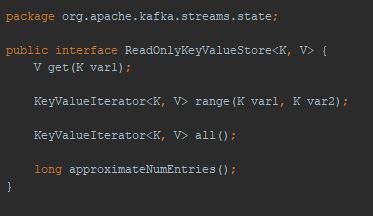
\includegraphics[width=0.7\textwidth]{images/ReadOnlyKeyValueStore.JPG}
  \caption{ReadOnlyKeyValueStore. Źródło: opracowanie własne }
\end{figure}
\FloatBarrier

Cała walidacja zostaje przeprowadzona w klasie ValidatorService w paczce  pl.cba.gibcode.apiCommand.service.
\begin{figure}[h!]
  \centering
    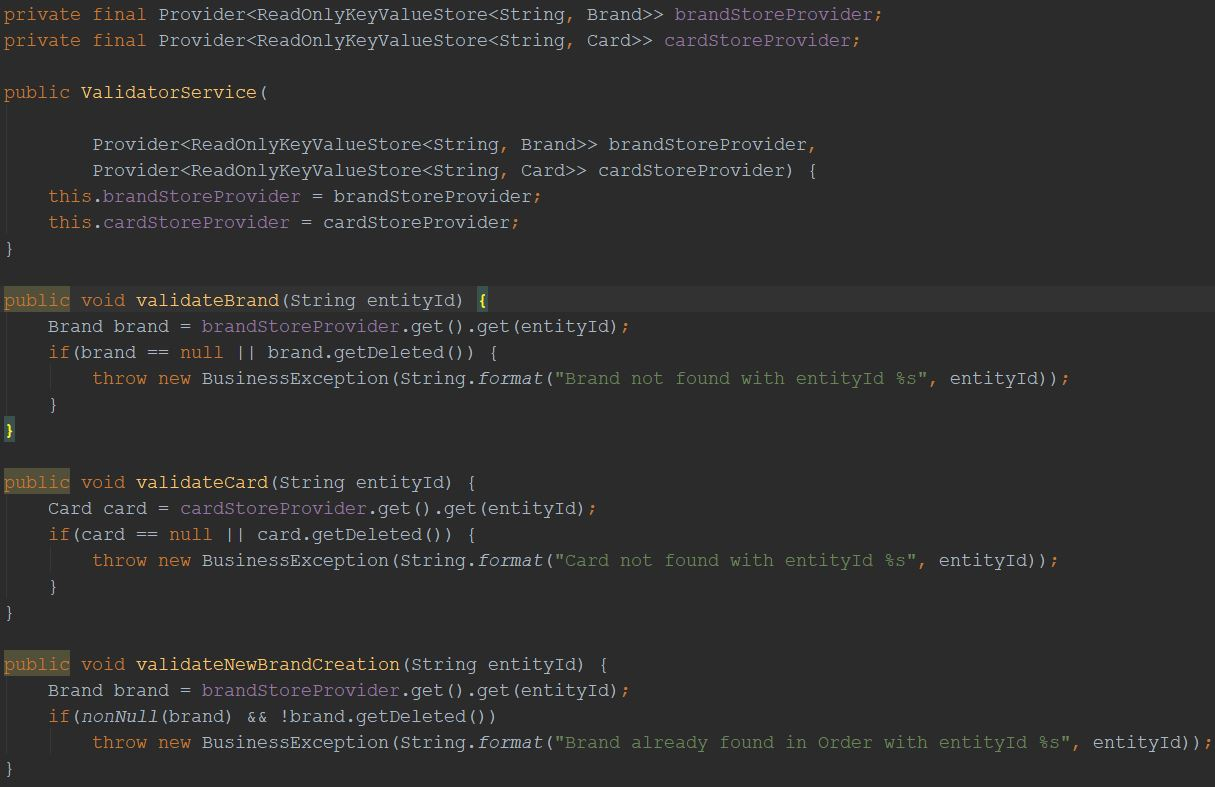
\includegraphics[width=1.0\textwidth]{images/ValidatorService.JPG}
  \caption{ValidatorService odpowiedzialny za walidacje nowych wydarzeń przed wysłaniem do Kafki. Źródło: opracowanie własne }
\end{figure}
\FloatBarrier

\subsection{Sposób użycia Kafka Producer API}

Po zwalidowaniu żądania pochodzącego z REST Api, apiCommand komunikuje się z brokerem za pomocą Kafka Producer API. Wiadomość, traktowana jako tworzące się nowe wydarzenie, zostaje wysłana, co jest równoznaczne z późniejszym stworzeniem zamówienia w systemie. Zamówienie zostaje wysłane przez Kafkę na temat ,,orderComponentEvent", który subksrybowany jest przez mikroserwis o nazwie orderComponent. Klasa SendService z pakietu pl.cba.gibcode.apiCommand.service odpowiedzialna jest za przygotowanie wydarzenia i wysłanie go przez Kafka Producer API. Klasa ma metody postOrder do tworzenia nowego zamówienia i putOrder do aktualizacji istniejącej karty lub marki.
\begin{figure}[h!]
  \centering
    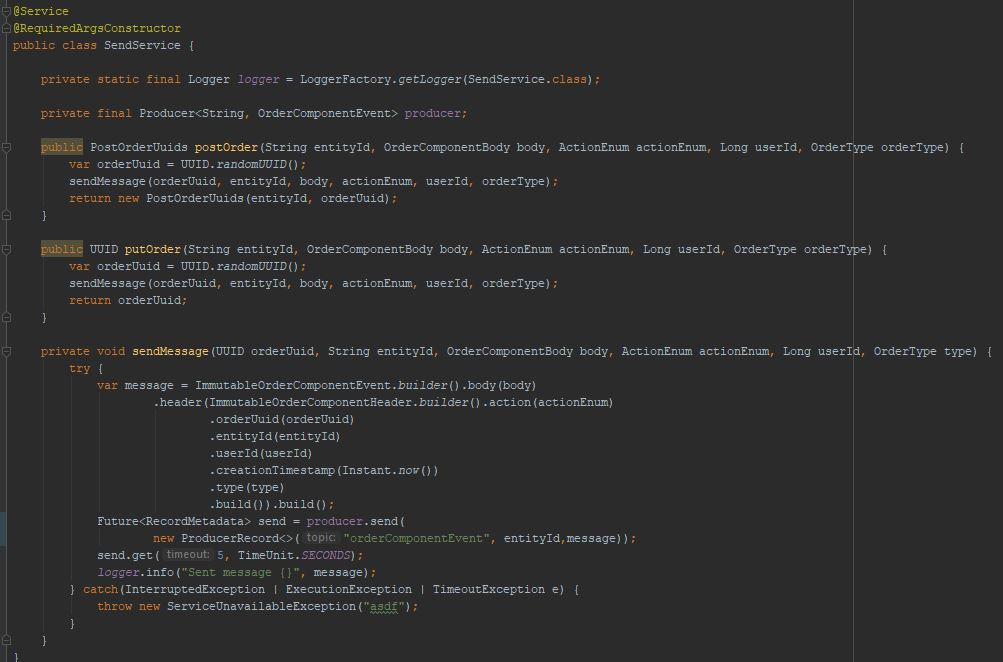
\includegraphics[width=1.0\textwidth]{images/SendService.JPG}
  \caption{SendService. Źródło: opracowanie własne }
\end{figure}
\FloatBarrier


\subsection{REST'owe Endpointy}
Każda funkcjonalność, tak jak w przypadku aplikacji w wersji monolitycznej\index{aplikacja monolityczna}, jest udostępniana przez REST Api i interfejs Swagger.
Ten mikroserwis udostępnia wszystkie funkcjonalności związane z operacjami zmieniającymi stan danych w aplikacji.

\begin{figure}[h!]
  \centering
    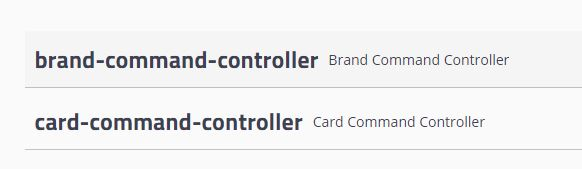
\includegraphics[width=0.7\textwidth]{images/controllerlistApiCommand.JPG}
  \caption{Lista kontrolerów w mikroserwisie apiCommand. Źródło: opracowanie własne }
\end{figure}
\FloatBarrier

\subsubsection{Kontroler Marki}
Kontroler wykonujący operacje komend na markach składa się z endpointów:
\begin{itemize}
    \item admin/brands jako HTTP PUT - aktualizacja marki przez administratora,
    \item admin/brands jako HTTP DELETE - usuwanie marki przez administratora,
    \item brands/create - tworzenie nowej marki,
\end{itemize}
\begin{figure}[h!]
  \centering
    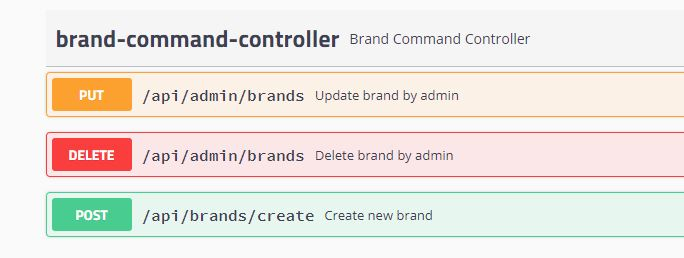
\includegraphics[width=1.0\textwidth]{images/brandContrApiCommand.JPG}
  \caption{Endpointy kontrolera marki. Źródło: opracowanie własne }
\end{figure}
\FloatBarrier
\subsubsection{Kontroler Kart}
Kontroler wykonujący operacje komend na kartach składa się z endpointów:
\begin{itemize}
    \item admin/cards jako HTTP DETELE - usuwanie karty z systemu przez administratora,
    \item admin/cards/validate - walidowanie karty przez administratora,
    \item buyer/checkout - dokonanie zamówienia przez kupującego,
    \item buyer/pay - dokonanie płatności przez kupującego,
    \item seller/card jako HTTP POST - tworzenie karty przez sprzedającego,
    \item seller/card jako HTTP PUT - aktualizacja karty przez sprzedającego,
    \item seller/card jako HTTP DELETE - usuwanie karty przez sprzedającego,
    \item seller/card/send - wysyłanie karty przez sprzedającego,
\end{itemize}
\begin{figure}[h!]
  \centering
    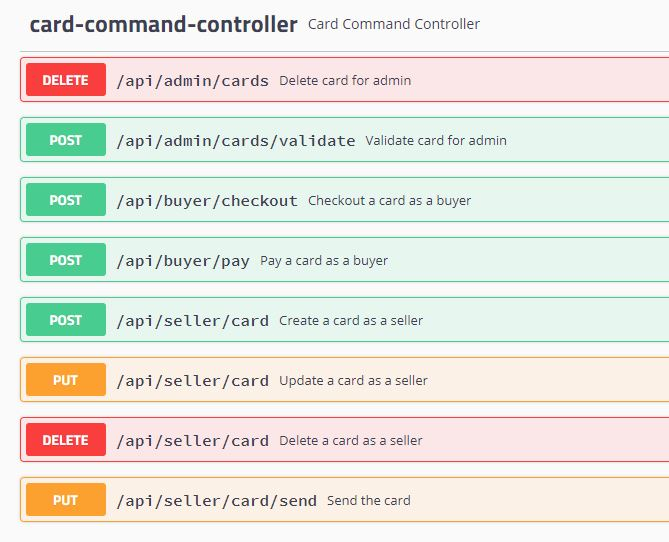
\includegraphics[width=1.0\textwidth]{images/cardContrApiCommand.JPG}
  \caption{Endpointy kontrolera kart. Źródło: opracowanie własne }
\end{figure}
\FloatBarrier
\subsection{Uruchomienie aplikacji}
Aby uruchomić aplikację trzeba mieć zainstalowany, tak jak w przypadku aplikacji monolitycznej\index{aplikacja monolityczna}, Apache Maven w wersji 3.
Następnie serwer Kafki musi zostać włączony i być dostępny pod adresem podanym w pliku application.properties, a domyślnie jest nim localhost:9092. Użytye zostało w tym celu Kafka Lenses ze strony \url{https://docs.lenses.io/install_setup/download.html} jako obraz dockerowy.
Po tym, w głównym folderze z kodem źródłowym należy podać komendę w terminalu ,,mvn spring-boot:run''. Ta komenda spowoduje, że aplikacja zostanie zbudowana i wystartuje na wbudowanym serwerze aplikacyjnym Tomcat na porcie 1000.

Aplikacja po uruchomieniu powinna być dostępna na \url{http://localhost:1000/ala-karta/swagger-ui.html}
Jest to strona z interfejsem udostępnionym przez Swaggera, gdzie można wykonywać interkaktywne zapytanie do udostępnionego REST Api.


\section{Struktura aplikacji apiQuery}
Aplikacja apiQuery, podobnie jak apiCommand, odpowiada za interakcję z interfejsem użytkownika poprzez przyjmowanie zapytań HTTP. Wystawiony jest własny REST Api. Ten mikroserwis odpowiada tylko i wyłącznie za odczytywanie stanu danych w systemie. Posiada definicję wszystkich operacji, które nie zmieniają stanu encji ani nie wykonują żadnych akcji na nich poza zczytywaniem. Po przyjęciu żądania HTTP aplikacja korzysta z ReadOnlyKeyValueStore w celu wyciągania informacji o encjach. Udostępniono możliwość filtrowania wyników a także podział danych na strony, gdzie zwracana jest tylko strona odpowiedzi (domyślnie 20 wpisów), co zmiejsza obciążenie sieci i poprawia szybkość przetwarzania żądania, a także pomaga w dogodnym zaprojektowaniu stronnicowania wyników w interfejsie użytkownika. Dane, które można zażądać przez apiQuery dotyczą stanu encji kart i marek a także jest możliwość zapytania o dane zamówienie (np. akcja usunięcia karty) czy zostało przeprowadzone pozytywnie i z jaką encją jest powiązane.

\subsection{Organizacja kodu}
Kod, tak jak w przypadku apiCommand ma logiczną strukturę składającą się z:
\begin{itemize}
    \item ,,config'' zawiera wszystkie pliki konfiguracyjne,
    \item ,,model'' zawiera wszystkie modele obiektów używane tylko i wyłącznie przez ten mikroserwis. Pozostałe modele wspólne są w osobnym module modelLibrary,
    \item ,,helper'' posiada klasę CriteriaBuilderHelper pomagającą tworzyć filtrowanie kart i marek,
    \item ,,service'' zawiera tzw. serwisy, czyli klasy posiadające logikę biznesową np. usuwanie karty z systemu,
    \item "web" to pakiet z kontrolerami Springowymi udostępniającymi zasoby przez REST Api.
\end{itemize}

\begin{figure}[h!]
  \centering
    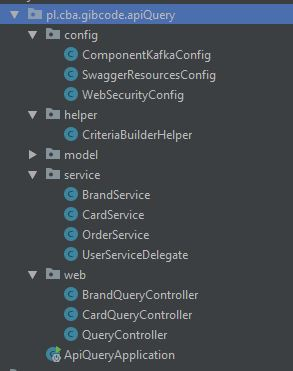
\includegraphics[width=0.5\textwidth]{images/apiQuery_packages.JPG}
  \caption{Organizacja kodu w apiQuery. Źródło: opracowanie własne }
\end{figure}
\FloatBarrier

\subsection{REST'owe endpointy}
Każda funkcjonalność, tak jak w przypadku aplikacji w wersji monolitycznej\index{aplikacja monolityczna}, jest udostępniana przez REST Api i interfejs Swagger.
Ten mikroserwis udostępnia wszystkie funkcjonalności związane z operacjami tylko i wyłącznie odczytującymi stan danych w aplikacji.

\subsubsection{Kontroler marek}
Kontrol wykonujący zapytania zczytujące stan encji marek. Posiada możliwość filtrowania i stronnicowania wyników.

\begin{itemize}
    \item admin/brands - lista wszystkich marek, w tym marek nieposiadających żadnej karty, czyli nieaktywnych w sprzedaży,
    \item brands/list - lista wszystkich aktywnych marek, których karty są do sprzedaży.
\end{itemize}

\subsubsection{Kontroler kart}
Kontroler wykonujący zapytania zczytujące stan encji kart. Posiada możliwość filtrowania i stronnicowania wyników.

\begin{itemize}
    \item admin/cards - lista wszystkich kart, w tym kart niezwalidowanych przez adminsitora, usuniętych lub uprzednio sprzedanych a także wysłanych,
    \item cards/list - lista wszystkich aktywnych kart będących dostępnymi w sprzedaży.
\end{itemize}

\subsubsection{Query kontroler}
Ogólny kontroler posiadający endpointy do sprawdzania stanów transakcji wykonywanych w systemie, a także informacji o aktualnym stanie danego zamówienia związanego z konkretnym wydarzeniem w systemie. Każda transackcja rozpoczyna się w momencie potwiedzenia złożenia zamówienia karty (ang. checkout) przez kupującego.

\begin{itemize}
    \item admin/transactions - lista wszystkich transakcji dla administratora,
    \item buyer/transactions - lista wszystkich transakcji dotycząca danego kupującego,
    \item orders - na podstawie orderUUID zwracane dane zamówienie (ang. order) i jego status. Mowa o zamówieniu jako wyniku wydarzenia w systemie, a nie o czynności potwiedzającej zamówienie (ang. checkout) karty,
    \item seller/transactions - lista wszystkich transakcji dotycząca danego sprzedającego.
\end{itemize}

\begin{figure}[h!]
  \centering
    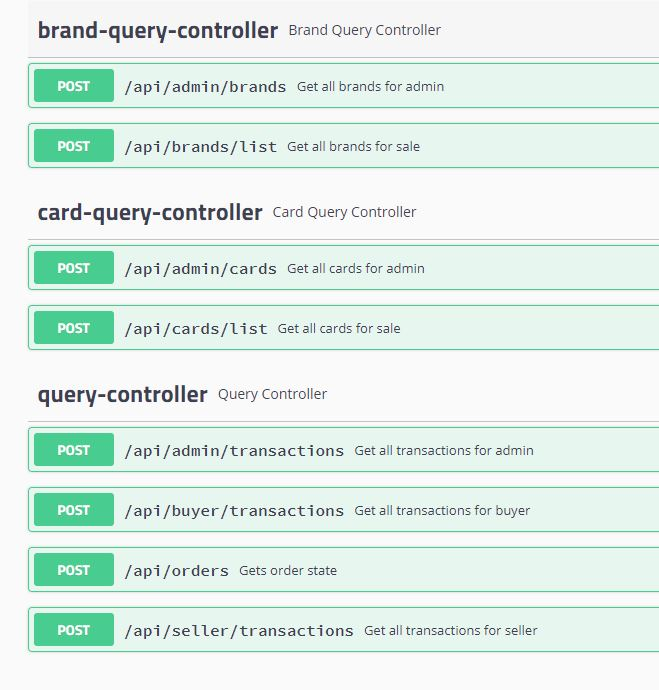
\includegraphics[width=0.7\textwidth]{images/controllerlistApiQuery.JPG}
  \caption{Lista kontrolerów i endpointów w mikroserwisie apiQuery. Źródło: opracowanie własne }
\end{figure}
\FloatBarrier

\subsection{Uruchomienie aplikacji}
Aby uruchomić aplikację trzeba mieć zainstalowany, tak jak w przypadku aplikacji monolitycznej\index{aplikacja monolityczna}, Apache Maven w wersji 3 i uruchomiony serwer Apache Kafka.
Po tym, w głównym folderze z kodem źródłowym należy podać komendę w terminalu ,,mvn spring-boot:run''. Ta komenda spowoduje, że aplikacja zostanie zbudowana i wystartuje na wbudowanym serwerze aplikacyjnym Tomcat na porcie 1002.

Aplikacja po uruchomieniu powinna być dostępna na \url{http://localhost:1002/ala-karta/swagger-ui.html}
Jest to strona z interfejsem udostępnionym przez Swaggera, gdzie można wykonywać interkaktywne zapytanie do udostępnionego REST Api.

\section{Struktura aplikacji orderComponent}
Mikroserwis orderComponent jest odpowiedzialny za przetwarzanie wydarzeń i tworzenie na ich podstawie zamówień w systemie (ang. order) związanych z daną akcją przesyłaną w nagłówku wiadomości. Aplikacja komunikuje się tylko i wyłącznie za pomocą wydarzeń poprzez broker Kafki. Po otrzymaniu wiadmości poprzez strumień Kafki dokonywane są wszystkie operacje na encjach, a także ich walidacja. Dla przykładu karta już sprzedana nie może zostać sprzedana ponownie. Aplikacja jest implementacją maszyny stanów, gdzie logika biznesowa jest oparta o możliwe stany encji w jakich mogą się znajdować. Jest weryfikowana, czy akcja na danej encji jest wykonywalna na podstawie definicji możliwych przejść między stanami encji w połączeniu z listą zezwolonych akcji.

Impementacja maszyny stanów znajduje się w klasie StateMachine w pakiecie pl.cba.gibcode.orderComponent.command.service.
\begin{figure}[h!]
  \centering
    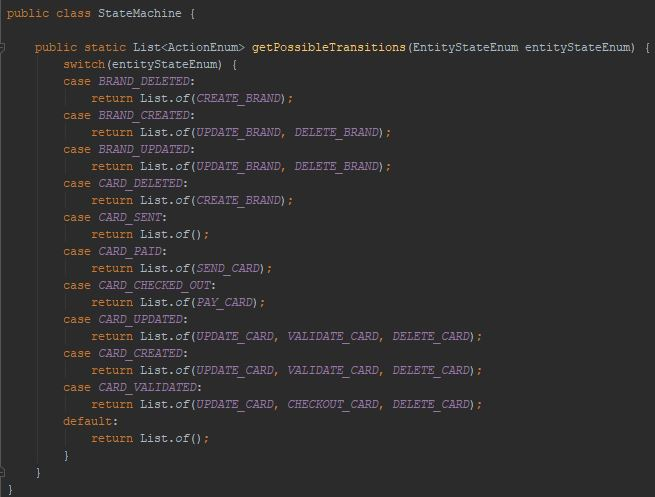
\includegraphics[width=1.0\textwidth]{images/StateMachine.JPG}
  \caption{Maszyna stanów. Źródło: opracowanie własne }
\end{figure}
\FloatBarrier

Kolejną ważną cechą tej aplikacji jest ekstensywne wykorzystanie Kafka Streams API co jest opisanie w kolejnej sekcji.

\subsection{Organizacja procesorów strumieni poprzez Streams API}
Główny rdzeń całego systemu opiera się na wykorzystaniu Kafka Streams API. 
Logika przetwarzania strumieni nie jest skomplikowana i znajduje się w dwóch klasach, zgodnie z założeniem CQRS\index{CQRS} gdzie jedna klasa to gałąź przetwarzania strumieni dla komend a druga dla kwerend tylko do odczytu.

\subsubsection{Topologia komend}
Cała definicja topologii strumieni opartych o Kafka Streams API dotyczących komend w systemie znajduje się w StreamingConfig w pakiecie pl.cba.gibcode.orderComponent.command.config. 

Aplikacja nasłuchuje na temat ,,orderComponentTopic'' i reaguje przy otrzymaniu wiadomości. Każda wiadomość jest traktowana jako wydarzenie w systemie.
\begin{figure}[h!]
  \centering
    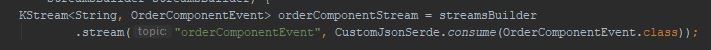
\includegraphics[width=1.0\textwidth]{images/streamscommand1.JPG}
  \caption{Subskrypcja tematu orderEventTopic jako początek przetwarzania strumieni. Źródło: opracowanie własne }
\end{figure}
\FloatBarrier

Wiadomość, którą otrzymujemy w strumieniu transformujemy przez logikę biznesową, gdzie rezultatem tego przetwarzania jest nowa informacja, którą wysyłamy na tematy ,,order'', ,,card'' i ,,brand''. Te tematy zawierają wszystkie informacje o encjach z nimi powiązanymi. Temat ,,order'' to zamówienie w systemie (nie mówimy o potwiedzenia zamówienia karty tylko o zamówieniu jako rezultacie jakiegokolwiek wydarzenia w aplikacji). Temat ,,card''dla kart i ,,brand'' dla marek. 

\begin{figure}[h!]
  \centering
    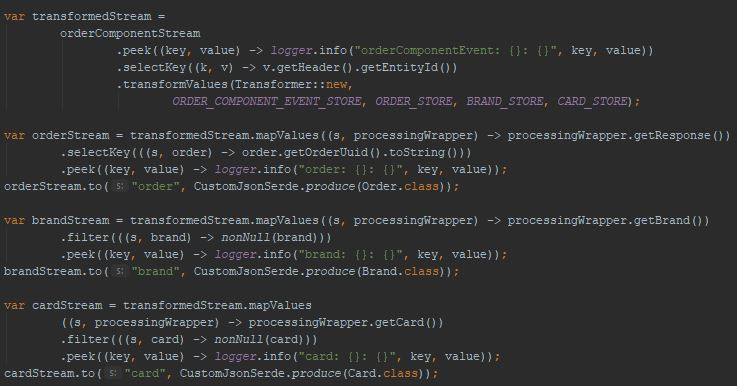
\includegraphics[width=1.0\textwidth]{images/streamscommand2.JPG}
  \caption{Transformacja i wysyłanie informacji na pojedynczy temat per encja. Źródło: opracowanie własne }
\end{figure}
\FloatBarrier

Transformacja przy użyciu zasad opisanych w logice biznesowej znajduje się w prywatnej klasie Transformer w obiekcie StreamingConfig. Jest tam m.in. walidowane wydarzenie w powiązaniu z daną akcją i typem, opierające się na logice maszyny stanów.

\begin{figure}[h!]
  \centering
    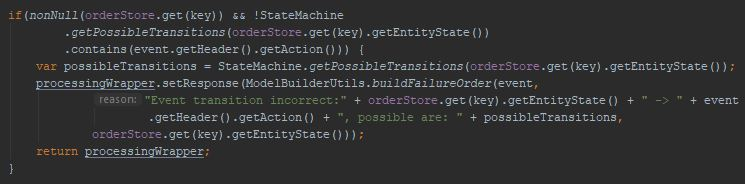
\includegraphics[width=1.0\textwidth]{images/streamscommand3.JPG}
  \caption{Walidacja możliwych przejść na podstawie maszyny stanów. Źródło: opracowanie własne }
\end{figure}
\FloatBarrier


Ostatnim krokiem w przetwarzaniu strumieni jest przygotowanie informacji dostępnych dla mikroserwisu apiQuery.
Dane, które są przygotowane dla kwerend, są obliczane na bieżąco przy każdym wydarzeniu. Wszystkie inne tematy znajdujące się w topologii Kafki zostają również wzbudzone i przetwarzane ponownie.
Jednym z przykładów użycia jest zapytanie o wszystkie karty na podstawie marki. Rezultat jest zapisywany na osobnym temacie, który jest w tym wypadku nazwany ,,queryCardsByBrand''.

\begin{figure}[h!]
  \centering
    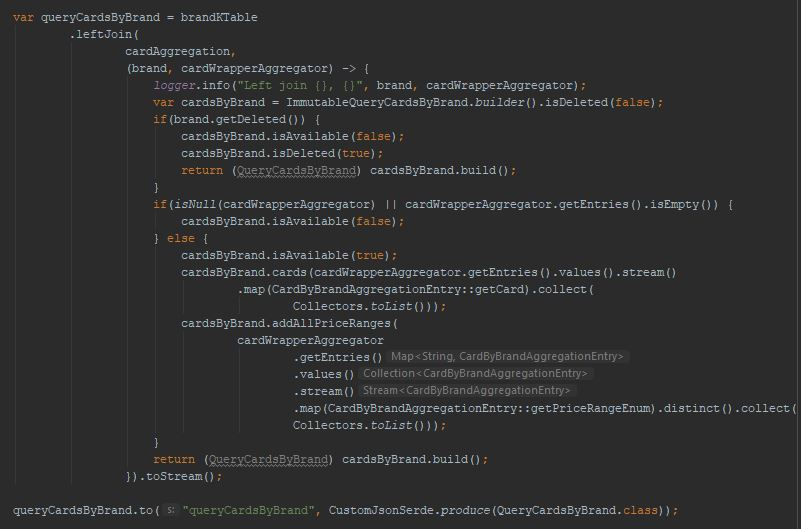
\includegraphics[width=1.0\textwidth]{images/streamsquery1.JPG}
  \caption{Agregacja listy kart na podstawie nazwy marki. Źródło: opracowanie własne }
\end{figure}
\FloatBarrier
\subsection{Organizacja kodu}
Podział kodu jest bardzo podobny do pozostałych mikroserwisów. Zgodnie z ideą CQRS\index{CQRS} pakiety zostały podzielone na cześć ,,command'' i część ,,query''. Dodatkowym pakietem jest ,,strategy'' gdzie zdefiniowane są wszystkie możliwe operacje w systemie.

\begin{figure}[h!]
  \centering
    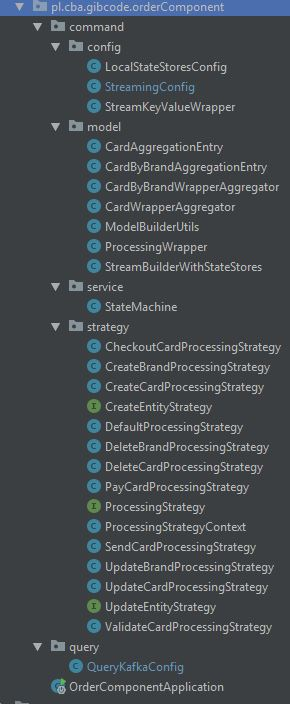
\includegraphics[width=0.5\textwidth]{images/orderComponent_packages.JPG}
  \caption{Organizacja kodu w orderComponent. Źródło: opracowanie własne }
\end{figure}
\FloatBarrier

\subsection{Uruchomienie aplikacji}
Aby uruchomić aplikację trzeba mieć zainstalowany Apache Maven w wersji 3 i uruchomiony serwer Apache Kafka.

Po tym, w głównym folderze z kodem źródłowym należy podać komendę w terminalu ,,mvn spring-boot:run''. Ta komenda spowoduje, że aplikacja zostanie zbudowana i wystartuje na wbudowanym serwerze aplikacyjnym Tomcat na porcie 1001.
Aplikacja nie ma żadnego interfejsu ani REST Api, w przeciwieństwie do apiQuery czy apiCommand.

Włączenie aplikacji po raz pierwszy przy połączeniu z brokerem Kafki wywołuje utworzenie tematów automatycznie.

\begin{figure}[h!]
  \centering
    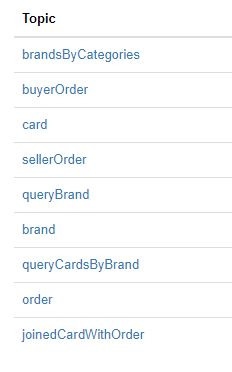
\includegraphics[width=0.5\textwidth]{images/tematy.JPG}
  \caption{Lista tematów w interfejsie Kafka Lenses. Źródło: opracowanie własne }
\end{figure}
\FloatBarrier